\documentclass{standalone}
\usepackage{tikz}
\usetikzlibrary{patterns, positioning}

\begin{document}
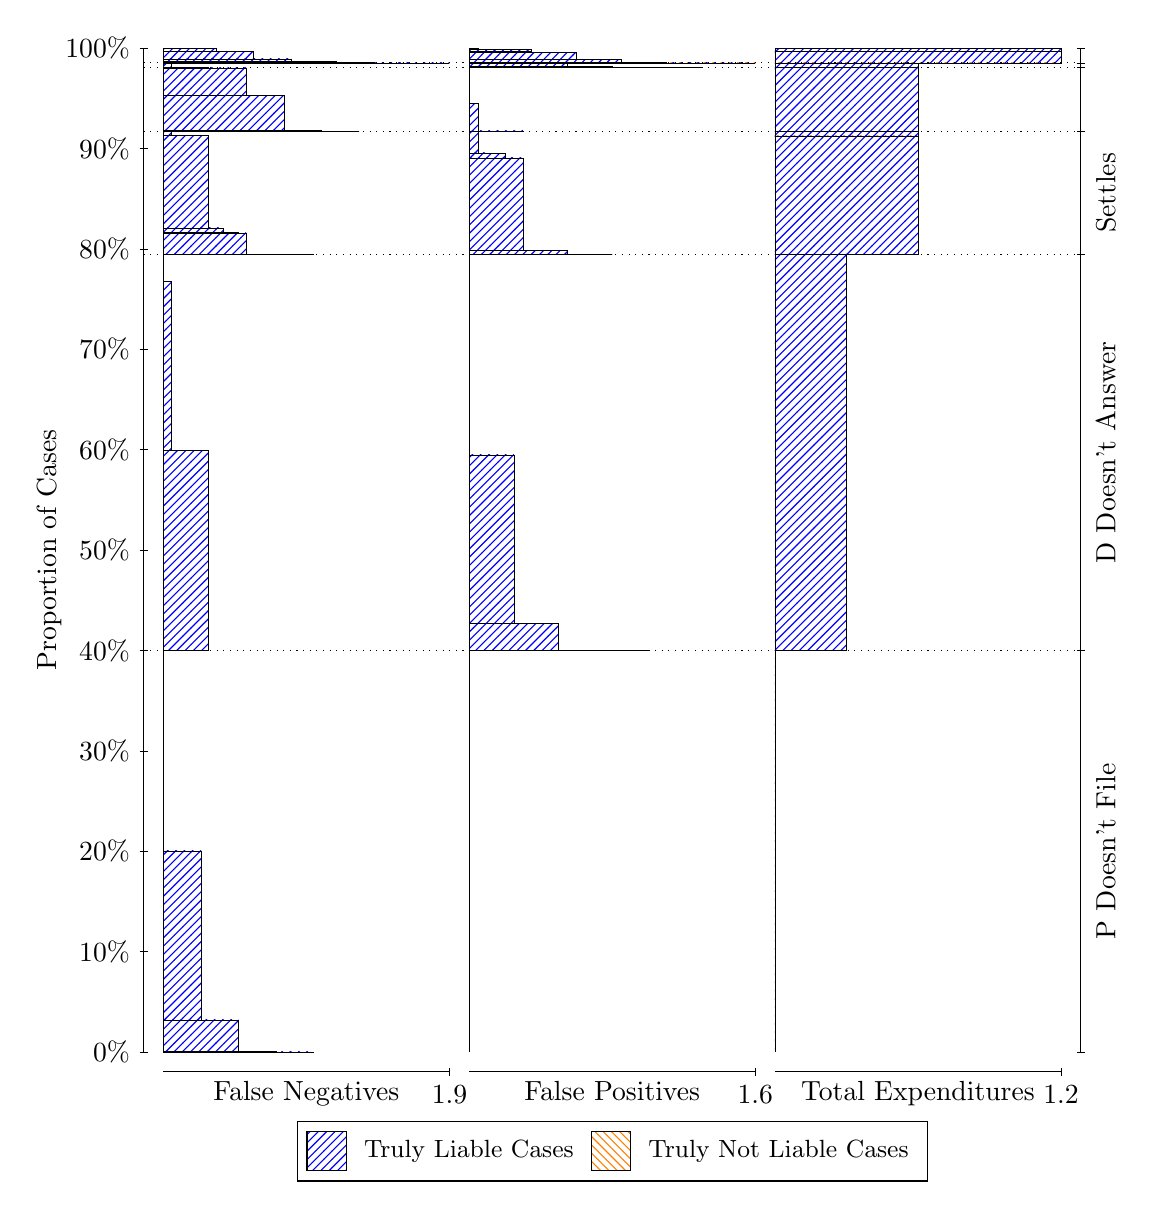
\begin{tikzpicture}
\draw[black, very thin] (1.5,1.75) -- (1.5,14.5);
\node[rotate=90, anchor=center] at (0.3, 8.125) {Proportion of Cases};
\draw[black, very thin] (1.45,1.75) -- (1.55,1.75);
\node[anchor=east] at (1.45, 1.75) {0\%};
\draw[black, very thin] (1.45,3.025) -- (1.55,3.025);
\node[anchor=east] at (1.45, 3.025) {10\%};
\draw[black, very thin] (1.45,4.3) -- (1.55,4.3);
\node[anchor=east] at (1.45, 4.3) {20\%};
\draw[black, very thin] (1.45,5.575) -- (1.55,5.575);
\node[anchor=east] at (1.45, 5.575) {30\%};
\draw[black, very thin] (1.45,6.85) -- (1.55,6.85);
\node[anchor=east] at (1.45, 6.85) {40\%};
\draw[black, very thin] (1.45,8.125) -- (1.55,8.125);
\node[anchor=east] at (1.45, 8.125) {50\%};
\draw[black, very thin] (1.45,9.4) -- (1.55,9.4);
\node[anchor=east] at (1.45, 9.4) {60\%};
\draw[black, very thin] (1.45,10.675) -- (1.55,10.675);
\node[anchor=east] at (1.45, 10.675) {70\%};
\draw[black, very thin] (1.45,11.95) -- (1.55,11.95);
\node[anchor=east] at (1.45, 11.95) {80\%};
\draw[black, very thin] (1.45,13.225) -- (1.55,13.225);
\node[anchor=east] at (1.45, 13.225) {90\%};
\draw[black, very thin] (1.45,14.5) -- (1.55,14.5);
\node[anchor=east] at (1.45, 14.5) {100\%};

\draw[black, very thin] (13.4,1.75) -- (13.4,14.5);
\draw[black, very thin] (13.35,1.75) -- (13.45,1.75);
\node[anchor=west] at (13.35, 1.75) {};
\draw[black, very thin] (13.35,6.8489) -- (13.45,6.8489);
\node[anchor=west] at (13.35, 6.8489) {};
\draw[black, very thin] (13.35,11.878) -- (13.45,11.878);
\node[anchor=west] at (13.35, 11.878) {};
\draw[black, very thin] (13.35,13.442) -- (13.45,13.442);
\node[anchor=west] at (13.35, 13.442) {};
\draw[black, very thin] (13.35,14.252) -- (13.45,14.252);
\node[anchor=west] at (13.35, 14.252) {};
\draw[black, very thin] (13.35,14.311) -- (13.45,14.311);
\node[anchor=west] at (13.35, 14.311) {};
\draw[black, very thin] (13.35,14.5) -- (13.45,14.5);
\node[anchor=west] at (13.35, 14.5) {};

\draw[black, very thin, pattern color=blue, pattern=north east lines] (1.75,1.75) rectangle (3.6623,1.75);
\draw[black, very thin, pattern color=blue, pattern=north east lines] (1.75,1.75) rectangle (3.1842,1.7534);
\draw[black, very thin, pattern color=blue, pattern=north east lines] (1.75,1.7534) rectangle (2.7061,2.158);
\draw[black, very thin, pattern color=blue, pattern=north east lines] (1.75,2.158) rectangle (2.2281,4.3029);
\draw[black, very thin, pattern color=orange, pattern=north west lines] (1.75,4.3029) rectangle (1.75,4.3029);
\draw[black, very thin, pattern color=blue, pattern=north east lines] (1.75,4.3029) rectangle (1.75,6.8489);
\draw[black, very thin, pattern color=blue, pattern=north east lines] (1.75,6.8489) rectangle (2.3237,9.3947);
\draw[black, very thin, pattern color=blue, pattern=north east lines] (1.75,9.3947) rectangle (1.8456,11.537);
\draw[black, very thin, pattern color=orange, pattern=north west lines] (1.75,11.537) rectangle (1.75,11.537);
\draw[black, very thin, pattern color=blue, pattern=north east lines] (1.75,11.537) rectangle (1.75,11.878);
\draw[black, very thin, pattern color=blue, pattern=north east lines] (1.75,11.878) rectangle (3.6623,11.878);
\draw[black, very thin, pattern color=blue, pattern=north east lines] (1.75,11.878) rectangle (3.4711,11.878);
\draw[black, very thin, pattern color=blue, pattern=north east lines] (1.75,11.878) rectangle (3.2798,11.878);
\draw[black, very thin, pattern color=blue, pattern=north east lines] (1.75,11.878) rectangle (3.1842,11.879);
\draw[black, very thin, pattern color=blue, pattern=north east lines] (1.75,11.879) rectangle (2.993,11.882);
\draw[black, very thin, pattern color=blue, pattern=north east lines] (1.75,11.882) rectangle (2.8018,12.152);
\draw[black, very thin, pattern color=blue, pattern=north east lines] (1.75,12.152) rectangle (2.7061,12.162);
\draw[black, very thin, pattern color=blue, pattern=north east lines] (1.75,12.162) rectangle (2.5149,12.215);
\draw[black, very thin, pattern color=blue, pattern=north east lines] (1.75,12.215) rectangle (2.3237,13.388);
\draw[black, very thin, pattern color=blue, pattern=north east lines] (1.75,13.388) rectangle (2.2281,13.388);
\draw[black, very thin, pattern color=blue, pattern=north east lines] (1.75,13.388) rectangle (2.0368,13.391);
\draw[black, very thin, pattern color=blue, pattern=north east lines] (1.75,13.391) rectangle (1.8456,13.442);
\draw[black, very thin, pattern color=orange, pattern=north west lines] (1.75,13.442) rectangle (1.75,13.442);
\draw[black, very thin, pattern color=blue, pattern=north east lines] (1.75,13.442) rectangle (1.75,13.442);
\draw[black, very thin, pattern color=blue, pattern=north east lines] (1.75,13.442) rectangle (4.236,13.442);
\draw[black, very thin, pattern color=blue, pattern=north east lines] (1.75,13.442) rectangle (3.7579,13.452);
\draw[black, very thin, pattern color=blue, pattern=north east lines] (1.75,13.452) rectangle (3.2798,13.901);
\draw[black, very thin, pattern color=blue, pattern=north east lines] (1.75,13.901) rectangle (2.8018,14.248);
\draw[black, very thin, pattern color=blue, pattern=north east lines] (1.75,14.248) rectangle (2.3237,14.252);
\draw[black, very thin, pattern color=orange, pattern=north west lines] (1.75,14.252) rectangle (1.75,14.252);
\draw[black, very thin, pattern color=blue, pattern=north east lines] (1.75,14.252) rectangle (2.3237,14.254);
\draw[black, very thin, pattern color=blue, pattern=north east lines] (1.75,14.254) rectangle (1.8456,14.3);
\draw[black, very thin, pattern color=orange, pattern=north west lines] (1.75,14.3) rectangle (1.75,14.3);
\draw[black, very thin, pattern color=blue, pattern=north east lines] (1.75,14.3) rectangle (1.75,14.311);
\draw[black, very thin, pattern color=blue, pattern=north east lines] (1.75,14.311) rectangle (5.3833,14.311);
\draw[black, very thin, pattern color=blue, pattern=north east lines] (1.75,14.311) rectangle (4.9053,14.311);
\draw[black, very thin, pattern color=blue, pattern=north east lines] (1.75,14.311) rectangle (4.4272,14.315);
\draw[black, very thin, pattern color=blue, pattern=north east lines] (1.75,14.315) rectangle (4.3316,14.315);
\draw[black, very thin, pattern color=blue, pattern=north east lines] (1.75,14.315) rectangle (3.9491,14.331);
\draw[black, very thin, pattern color=blue, pattern=north east lines] (1.75,14.331) rectangle (3.8535,14.331);
\draw[black, very thin, pattern color=blue, pattern=north east lines] (1.75,14.331) rectangle (3.4711,14.333);
\draw[black, very thin, pattern color=blue, pattern=north east lines] (1.75,14.333) rectangle (3.3754,14.361);
\draw[black, very thin, pattern color=blue, pattern=north east lines] (1.75,14.361) rectangle (2.993,14.361);
\draw[black, very thin, pattern color=blue, pattern=north east lines] (1.75,14.361) rectangle (2.8974,14.454);
\draw[black, very thin, pattern color=blue, pattern=north east lines] (1.75,14.454) rectangle (2.5149,14.454);
\draw[black, very thin, pattern color=blue, pattern=north east lines] (1.75,14.454) rectangle (2.4193,14.497);
\draw[black, very thin, pattern color=blue, pattern=north east lines] (1.75,14.497) rectangle (1.9412,14.5);
\draw[black, very thin, pattern color=orange, pattern=north west lines] (1.75,14.5) rectangle (1.75,14.5);
\draw[black, very thin, pattern color=blue, pattern=north east lines] (1.75,14.5) rectangle (1.75,14.5);
\draw[black, very thin, pattern color=orange, pattern=north west lines] (5.6333,1.75) rectangle (5.6333,1.75);
\draw[black, very thin, pattern color=blue, pattern=north east lines] (5.6333,1.75) rectangle (5.6333,6.8489);
\draw[black, very thin, pattern color=orange, pattern=north west lines] (5.6333,6.8489) rectangle (7.9042,6.8489);
\draw[black, very thin, pattern color=blue, pattern=north east lines] (5.6333,6.8489) rectangle (7.9042,6.8489);
\draw[black, very thin, pattern color=blue, pattern=north east lines] (5.6333,6.8489) rectangle (7.3365,6.8494);
\draw[black, very thin, pattern color=blue, pattern=north east lines] (5.6333,6.8494) rectangle (6.7687,7.1898);
\draw[black, very thin, pattern color=blue, pattern=north east lines] (5.6333,7.1898) rectangle (6.201,9.3318);
\draw[black, very thin, pattern color=blue, pattern=north east lines] (5.6333,9.3318) rectangle (5.6333,11.878);
\draw[black, very thin, pattern color=orange, pattern=north west lines] (5.6333,11.878) rectangle (7.45,11.878);
\draw[black, very thin, pattern color=blue, pattern=north east lines] (5.6333,11.878) rectangle (7.45,11.878);
\draw[black, very thin, pattern color=orange, pattern=north west lines] (5.6333,11.878) rectangle (7.2229,11.878);
\draw[black, very thin, pattern color=blue, pattern=north east lines] (5.6333,11.878) rectangle (7.2229,11.878);
\draw[black, very thin, pattern color=orange, pattern=north west lines] (5.6333,11.878) rectangle (6.9958,11.878);
\draw[black, very thin, pattern color=blue, pattern=north east lines] (5.6333,11.878) rectangle (6.9958,11.878);
\draw[black, very thin, pattern color=blue, pattern=north east lines] (5.6333,11.878) rectangle (6.8823,11.929);
\draw[black, very thin, pattern color=blue, pattern=north east lines] (5.6333,11.929) rectangle (6.6552,11.932);
\draw[black, very thin, pattern color=blue, pattern=north east lines] (5.6333,11.932) rectangle (6.4281,11.932);
\draw[black, very thin, pattern color=blue, pattern=north east lines] (5.6333,11.932) rectangle (6.3146,13.105);
\draw[black, very thin, pattern color=blue, pattern=north east lines] (5.6333,13.105) rectangle (6.0875,13.158);
\draw[black, very thin, pattern color=blue, pattern=north east lines] (5.6333,13.158) rectangle (5.8604,13.168);
\draw[black, very thin, pattern color=blue, pattern=north east lines] (5.6333,13.168) rectangle (5.7469,13.439);
\draw[black, very thin, pattern color=blue, pattern=north east lines] (5.6333,13.439) rectangle (5.6333,13.442);
\draw[black, very thin, pattern color=orange, pattern=north west lines] (5.6333,13.442) rectangle (6.3146,13.442);
\draw[black, very thin, pattern color=blue, pattern=north east lines] (5.6333,13.442) rectangle (6.3146,13.447);
\draw[black, very thin, pattern color=blue, pattern=north east lines] (5.6333,13.447) rectangle (5.7469,13.794);
\draw[black, very thin, pattern color=blue, pattern=north east lines] (5.6333,13.794) rectangle (5.6333,14.252);
\draw[black, very thin, pattern color=orange, pattern=north west lines] (5.6333,14.252) rectangle (8.5854,14.252);
\draw[black, very thin, pattern color=blue, pattern=north east lines] (5.6333,14.252) rectangle (8.5854,14.252);
\draw[black, very thin, pattern color=blue, pattern=north east lines] (5.6333,14.252) rectangle (8.0177,14.252);
\draw[black, very thin, pattern color=blue, pattern=north east lines] (5.6333,14.252) rectangle (7.45,14.262);
\draw[black, very thin, pattern color=blue, pattern=north east lines] (5.6333,14.262) rectangle (6.8823,14.309);
\draw[black, very thin, pattern color=blue, pattern=north east lines] (5.6333,14.309) rectangle (6.3146,14.311);
\draw[black, very thin, pattern color=orange, pattern=north west lines] (5.6333,14.311) rectangle (9.2667,14.311);
\draw[black, very thin, pattern color=blue, pattern=north east lines] (5.6333,14.311) rectangle (9.2667,14.311);
\draw[black, very thin, pattern color=orange, pattern=north west lines] (5.6333,14.311) rectangle (8.699,14.311);
\draw[black, very thin, pattern color=blue, pattern=north east lines] (5.6333,14.311) rectangle (8.699,14.311);
\draw[black, very thin, pattern color=orange, pattern=north west lines] (5.6333,14.311) rectangle (8.1313,14.311);
\draw[black, very thin, pattern color=blue, pattern=north east lines] (5.6333,14.311) rectangle (8.1313,14.313);
\draw[black, very thin, pattern color=blue, pattern=north east lines] (5.6333,14.313) rectangle (7.5635,14.357);
\draw[black, very thin, pattern color=orange, pattern=north west lines] (5.6333,14.357) rectangle (7.5635,14.357);
\draw[black, very thin, pattern color=blue, pattern=north east lines] (5.6333,14.357) rectangle (7.5635,14.357);
\draw[black, very thin, pattern color=orange, pattern=north west lines] (5.6333,14.357) rectangle (7.45,14.357);
\draw[black, very thin, pattern color=blue, pattern=north east lines] (5.6333,14.357) rectangle (7.45,14.357);
\draw[black, very thin, pattern color=blue, pattern=north east lines] (5.6333,14.357) rectangle (6.9958,14.448);
\draw[black, very thin, pattern color=blue, pattern=north east lines] (5.6333,14.448) rectangle (6.9958,14.449);
\draw[black, very thin, pattern color=orange, pattern=north west lines] (5.6333,14.449) rectangle (6.8823,14.449);
\draw[black, very thin, pattern color=blue, pattern=north east lines] (5.6333,14.449) rectangle (6.8823,14.449);
\draw[black, very thin, pattern color=blue, pattern=north east lines] (5.6333,14.449) rectangle (6.4281,14.463);
\draw[black, very thin, pattern color=blue, pattern=north east lines] (5.6333,14.463) rectangle (6.4281,14.478);
\draw[black, very thin, pattern color=blue, pattern=north east lines] (5.6333,14.478) rectangle (6.3146,14.48);
\draw[black, very thin, pattern color=orange, pattern=north west lines] (5.6333,14.48) rectangle (6.3146,14.48);
\draw[black, very thin, pattern color=blue, pattern=north east lines] (5.6333,14.48) rectangle (6.3146,14.48);
\draw[black, very thin, pattern color=blue, pattern=north east lines] (5.6333,14.48) rectangle (5.8604,14.48);
\draw[black, very thin, pattern color=blue, pattern=north east lines] (5.6333,14.48) rectangle (5.8604,14.48);
\draw[black, very thin, pattern color=blue, pattern=north east lines] (5.6333,14.48) rectangle (5.7469,14.495);
\draw[black, very thin, pattern color=blue, pattern=north east lines] (5.6333,14.495) rectangle (5.7469,14.496);
\draw[black, very thin, pattern color=blue, pattern=north east lines] (5.6333,14.496) rectangle (5.6333,14.5);
\draw[black, very thin, pattern color=orange, pattern=north west lines] (9.5167,1.75) rectangle (9.5167,1.75);
\draw[black, very thin, pattern color=blue, pattern=north east lines] (9.5167,1.75) rectangle (9.5167,6.8489);
\draw[black, very thin, pattern color=orange, pattern=north west lines] (9.5167,6.8489) rectangle (10.425,6.8489);
\draw[black, very thin, pattern color=blue, pattern=north east lines] (9.5167,6.8489) rectangle (10.425,11.878);
\draw[black, very thin, pattern color=orange, pattern=north west lines] (9.5167,11.878) rectangle (11.333,11.878);
\draw[black, very thin, pattern color=blue, pattern=north east lines] (9.5167,11.878) rectangle (11.333,13.373);
\draw[black, very thin, pattern color=orange, pattern=north west lines] (9.5167,13.373) rectangle (11.333,13.373);
\draw[black, very thin, pattern color=blue, pattern=north east lines] (9.5167,13.373) rectangle (11.333,13.384);
\draw[black, very thin, pattern color=orange, pattern=north west lines] (9.5167,13.384) rectangle (11.333,13.384);
\draw[black, very thin, pattern color=blue, pattern=north east lines] (9.5167,13.384) rectangle (11.333,13.442);
\draw[black, very thin, pattern color=orange, pattern=north west lines] (9.5167,13.442) rectangle (11.333,13.442);
\draw[black, very thin, pattern color=blue, pattern=north east lines] (9.5167,13.442) rectangle (11.333,14.252);
\draw[black, very thin, pattern color=orange, pattern=north west lines] (9.5167,14.252) rectangle (11.333,14.252);
\draw[black, very thin, pattern color=blue, pattern=north east lines] (9.5167,14.252) rectangle (11.333,14.311);
\draw[black, very thin, pattern color=orange, pattern=north west lines] (9.5167,14.311) rectangle (13.15,14.311);
\draw[black, very thin, pattern color=blue, pattern=north east lines] (9.5167,14.311) rectangle (13.15,14.461);
\draw[black, very thin, pattern color=orange, pattern=north west lines] (9.5167,14.461) rectangle (13.15,14.461);
\draw[black, very thin, pattern color=blue, pattern=north east lines] (9.5167,14.461) rectangle (13.15,14.5);
\draw[black, dotted] (1.5,6.8489) -- (13.4,6.8489);
\draw[black, dotted] (1.5,11.878) -- (13.4,11.878);
\draw[black, dotted] (1.5,13.442) -- (13.4,13.442);
\draw[black, dotted] (1.5,14.252) -- (13.4,14.252);
\draw[black, dotted] (1.5,14.311) -- (13.4,14.311);
\draw[black, very thin] (1.75,1.5) -- (5.3833,1.5);
\node[anchor=north] at (3.5667, 1.5) {False Negatives};
\draw[black, very thin] (5.3833,1.45) -- (5.3833,1.55);
\node[anchor=north] at (5.3833, 1.45) {1.9};

\draw[black, very thin] (5.6333,1.5) -- (9.2667,1.5);
\node[anchor=north] at (7.45, 1.5) {False Positives};
\draw[black, very thin] (9.2667,1.45) -- (9.2667,1.55);
\node[anchor=north] at (9.2667, 1.45) {1.6};

\draw[black, very thin] (9.5167,1.5) -- (13.15,1.5);
\node[anchor=north] at (11.333, 1.5) {Total Expenditures};
\draw[black, very thin] (13.15,1.45) -- (13.15,1.55);
\node[anchor=north] at (13.15, 1.45) {1.2};

\node[black, centered, rotate=90] at (13.72, 4.2994) {P Doesn't File};
\node[black, centered, rotate=90] at (13.72, 9.3632) {D Doesn't Answer};
\node[black, centered, rotate=90] at (13.72, 12.66) {Settles};




\draw (7.449999999999999,1.5) node[draw=none] (baseCoordinate) {};
\begin{scope}[align=center]
        \matrix[scale=0.5, draw=black, below=0.5cm of baseCoordinate, nodes={draw}, column sep=0.1cm]{
            \node[rectangle, draw, minimum width=0.5cm, minimum height=0.5cm, pattern=north east lines, pattern color=blue] {}; &
            \node[draw=none, font=\small] (B) {Truly Liable Cases}; &
            \node[rectangle, draw, minimum width=0.5cm, minimum height=0.5cm, pattern=north west lines, pattern color=orange] {}; &
            \node[draw=none, font=\small] (B) {Truly Not Liable Cases}; \\
            };
\end{scope}

\end{tikzpicture}
\end{document}